\documentclass{article}
%\documentclass[man]{apa6}

\title{Detecting hysteresis in psychological processes with the hysteretic threshold autoregressive (HysTAR) model}
%\shorttitle{Detecting hysteresis with the HysTAR model}
\author{Daan de Jong, Ois\'{i}n Ryan, Han L.J. van der Maas, Ellen L. Hamaker}

%Layout
\usepackage{setspace}%\onehalfspacing
\usepackage{titlesec}
%\titleformat{\section}[wrap]{\normalfont\bfseries}{\thesection.}{0.5em}{}
\usepackage{fancyhdr}
%\fancyhead[L]{Title}
\fancyfoot[C]{\thepage}
\usepackage{multicol}
\usepackage{multirow}
\setlength{\columnsep}{1cm}
\usepackage[dvipsnames, table]{xcolor}
\usepackage{setspace, caption}
\usepackage{tabularx}
\DeclareCaptionLabelSeparator*{spaced}{\\[2ex]}
\captionsetup[table, figure]{textfont=it,format=plain,justification=justified,
  singlelinecheck=false,labelsep=spaced,skip=0pt}
%\captionsetup[figure]{labelsep=period,labelfont=it,justification=justified,
% singlelinecheck=false,font=doublespacing}

%Graphics
\usepackage{graphicx}
\graphicspath{ {./img/} }
\DeclareGraphicsExtensions{.pdf,.png}
\usepackage{tikz}
\usetikzlibrary{calc}
\usetikzlibrary{positioning}
\usepackage{pgflibraryarrows} 
\usepackage{pgflibrarysnakes}

%Links
\usepackage{hyperref}
\hypersetup{
    colorlinks=true,
    citecolor=BlueGreen,
    linkcolor=BlueGreen,
    filecolor=BlueGreen,      
    urlcolor=BlueGreen,
}

%References
\usepackage{apacite}
\usepackage{natbib}

%General
\usepackage{amsmath}
\usepackage{amssymb}
\usepackage{caption}
\usepackage{subcaption}
\usepackage{rotating}

%Commands
\newcommand{\N}{\mathbb{N}} %set of natural numbers
\newcommand{\Z}{\mathbb{Z}} %set of integers
\newcommand{\Q}{\mathbb{Q}} %set of rational numbers
\newcommand{\R}{\mathbb{R}} %set of real numbers
\newcommand{\C}{\mathbb{C}} %set of complex numbers
\newcommand{\V}[1]{\mathbf{#1}} %vector boldface notation
\newcommand{\prob}{\mathbb{P}}
\newcommand{\E}{\mathbb{E}}
\newcommand{\D}[1]{\mathrm{d}#1}
\newcommand{\var}{\mathrm{var}}
\DeclareMathOperator*{\argmin}{argmin}

%=======================================================================
\begin{document}
%\begin{multicols}{2}

%\input{front}
\maketitle


Abstract:
\textit{
Many psychological processes consist of different states or regimes, which are characterized by, for instance, different means and/or variances. 
Switches between these regimes are sometimes characterized by hysteresis, which makes a switch from one regime to another regime difficult to reverse. 
In the current study, we present the hysteretic threshold autoregressive (HysTAR) model, which can be used to detect hysteresis in a bivariate time series consisting of a control variable and an outcome variable. 
We created a user-friendly package in \textsf{R} to simulate data the HysTAR model and estimate its parameters. 
Estimation and model selection performance is investigated in simulation studies. 
Additionally, we further demonstrate the use of the HysTAR model with a time series of depression scores generated from a network of depression symptoms and with an empirical example on hysteresis in the speed-accuracy trade-off.
}

Keywords: \textit{hysteresis, regime switching, non-lineairity, bimodality, bistability, dynamical systems, threshold autoregression, intensive longitudinal data, time series analysis}
\newpage
\section{Introduction}
Individuals are complex dynamical systems, whose emotions, cognitions and behaviors constantly change over time.
To study the dynamics of their psychological processes, reseachers often measure these individuals at relatively many occasions that are typically closely spaced in time \citep{bolger2013intensive, walls2006models}.
The data resulting from these measurements are called \textit{intensive longitudinal data} (ILD) or \textit{time series data}, roughly defined to consist of at least 20 measurement occasions.
Technological advances have caused a enourmous growth in the collection of ILD with the use of ecogical momentary assessments, experience sampling and daily diaries \citep{notimelikethepresent}, resulting in a body of data containing a rich source of information about individual processes.
However, this source of information remains largely untapped when using conventional statistical models like the autoregressive model of order 1 (AR(1)). These models are often too restrictive to capture the inherently complex dynamics underpinning psychological phenomena, since they imply a symmetric distribution with a constant mean, variance and temporal associations between measurements \citep{box_jenkins, chatfield}.
However, it is evident that many psychological time series data exhibit nonstandard features, such as skewness \citep{skewness_oisin, skewness_2, skewness_3}, time-varying temporal associations \citep{changing_inertia_1, changing_inertia_2} and bimodality \citep{skewness_oisin, bimodality_han}.
The inadequacy of AR models in capturing these features has underscored the necessity for alternative modeling approaches.

In the current paper, we focus on modeling approaches to account for bimodality and jumps in psychological processes.
By bimodality, we simply mean that the distribution of the variable of interest has two modes.
From a dynamical systems perspective, these two modes of the variable of interest correspond to two \textit{stable equilibrium states} or two \textit{regimes} of the underlying system.
A stable equilibrium state is a state of the system at which it settles in the long run and returns to after small perturbations.
A regime is a closely related concept and refers to a specific pattern of behavior exhibited by the system over an extended period of time, and can be characterized by the stable equilibrium state that the system moves around and/or the rate at which this happens.
Jumps refer to large sudden changes in the variable of interest.
These changes occur at a state transition or regime switch, when the system ``jumps'' from one stable equilibrium state to another.

One class of models that was developed to account for bimodality and large sudden changes is formed by threshold autoregressive (TAR) models \citep{tar}.
In these time series models, the variable of interest falls within a certain regime at each point in time. 
The value of a \textit{control variable} determines which regime this is. 
When the control variable crosses a certain \textit{threshold}, the system shifts to another regime.
For example, the control variable temperature can push a system of water molecules from a solid into a liquid regime, when it crosses a threshold of 0 degrees Celsius.

But TAR models fail to account for an interesting regime-swichting phenomenon, however, the phenomenon of hysteresis. 
Hysteresis is present when the switches between two regimes are associated with two different thresholds, one for each direction of the state transition \citep{gilmore, strogatz}.
As a simple example, under high pressure, water freezes at -4 degrees Celsius and melts at 0 degrees Celcius, so there is a different temperature threshold for the transition from solid to liquid. As a result, a regime switch cannot be reversed as easy as would be the case when there is a single threshold (when water would have freezed and melted at 0 degrees Celsius, for example).
This irreversibility of hysteresic switches has intrigued researchers from fields like magnetics, biologiy, ecology, economy, sociology and psychology for a long time \citep{hysteresis_mathematical}.

Currently, hysteresis is often modeled with the (stochastic) cusp catastrophe model. Since this model uses differential equations to describe the system's dynamics, it is quite a challenge to fit this model to intensive longitudinal data \citep{cobb, CT_limitations1, CT_limitations2, R_cusp}. 
Instead, the cusp catastrophe model is often fit to cross-sectional data \citep[e.g.,][]{cusp_example_1, cusp_example_2, cusp_example_3}, which heavily impedes any conclusion about dynamics at the individual level \citep{molenaar_manifesto, hamaker_within}.
As a result, not much is known about hysteresis in psychological processes, yet.

Fortunately, a straightforward adaptation to the TAR model that incorporates the hysteresis effect was recently developed in the field of econometrics \citep{bar2}, resulting in the hysteretic TAR (HysTAR) model.
In the current paper, we bring the HysTAR model to the psychological realm in an accessible manner, opening up the possibility to study how hysteretic processes unfold over time, using intensive longitudinal data.

This paper is structured as follows.
In the next section, we introduce the concept of hysteresis.
In Section \ref{sec:LS_estimation}, we present the conditional least squares method to estimate the HysTAR model parameters, which was implemented by the first author in the accompanying \textsf{R}-package \texttt{hystar} \citep{R, R_hystar}.
In Section \ref{sec:simulation_study_1}, we conduct a simulation study to investigate whether hysteresis can be detected with model selection tools.
In Section \ref{sec:simulation_study_2}, we present another simulation study, focussed on estimation of the threshold parameters.
In Section \ref{sec:empirical_example_1}, we generate time series data from an empirical network of depression symptoms. Here, the research question is whether the HysTAR model can detect the hysteresis effect in the regime switches of this network.
Another empricial example is given in Section \ref{sec:empirical_illustration}, where the use of the HysTAR model is demonstrated in an analysis of the speed-accuracy trade-off phenomenon.
We conclude with a discussion section where we highlight current and future extensions to the HysTAR model.

\section{The hysteretic threshold autoregressive (HysTAR) model} \label{sec:hystar}
In this section, we will first introduce the standard threshold autoregressive (TAR) model.
Subsequently, we will explain how the TAR model can be expanded to the hysteretic TAR model to account for the hysteresis effect.

\subsection{TAR model}
The TAR model is a discrete time series model using piece-wise linearization to approximate non-linear features in the data, like bimodality and sudden jumps \citep{tar}.
This approach yields a very flexible, interpretable but still accurate description of the process at hand, which is one of the reasons why TAR models are so popular and widely applied in economics \citep{tar_in_economics}.
In psychology, the TAR model has been applied to capture sudden shifts in affect regulation within individuals \citep{tar_affect_person1, tar_affect_person2} and dyads \citep{tar_affect_dyadic1, tar_affect_dyadic2}.
In the two-regime TAR model \citet{tar}, an outcome variable $y$ follows an autoregressive process according to one of the regimes $R_t$ at each time $t = 0, 1, \dots, T$:

\begin{equation}
y_t = 
\begin{cases}
\phi_{00} + \phi_{01} y_{t-1} + \cdots + \phi_{0 p_0} y_{t-p_0} + \sigma_{0} \varepsilon_t & \text{if}~R_{t} = 0\\
\phi_{10} + \phi_{11} y_{t-1} + \cdots + \phi_{1 p_1} y_{t-p_1} + \sigma_{1} \varepsilon_t & \text{if}~R_{t} = 1, \\
\end{cases}
\label{eqn:ar_processes}
\end{equation}

where the residuals $\varepsilon_t$ have a mean of 0 and a variance of 1, and are all uncorrelated with each other.
Note that all AR parameters are allowed to differ between regimes: the intercept $\phi_{j0}$, the autoregressive coefficients $\phi_{j1}, \dots, \phi_{j p_j}$ and the residual standard deviations $\sigma_j$, where $j$ denotes the regime and $p_j$ denotes the order of the AR process, that is, the largest lag that is used in the prediction of $y_t$.
In this way, regimes can differ in their mean, temporal dynamics, and residual variance.
The long-run mean of $y$ in regime $j$ is given by $\phi_{j0}/(1 - \sum_{i=1}^{p_j} \phi_{ji})$. 
The dynamics are described by the autoregressive coefficients, that indicate the extent to which current and past values of $y$ are carried over to future observations.
Additionally, regime differences in $\sigma$ can indicate different associations between $y$ and unmeasured variables, or different amounts of measurement error.

How the process switches between regimes is dictated by the following equation:
\begin{equation} \label{eqn:simple_switching}
R_t = \begin{cases}
0 & \mathrm{if} \, z_{t-d} \le r \\
1 & \mathrm{if} \, z_{t-d} > r, \\
\end{cases}
\end{equation}

where $z$ denotes the control variable, $d$ is a positive integer allowing for a delayed effect of $z$ and $r$ is the threshold parameter. The left panel of Figure \ref{fig:simple_vs_hysteretic_2} illustrates how the regime is related to the control variable.

\begin{figure}
\centering
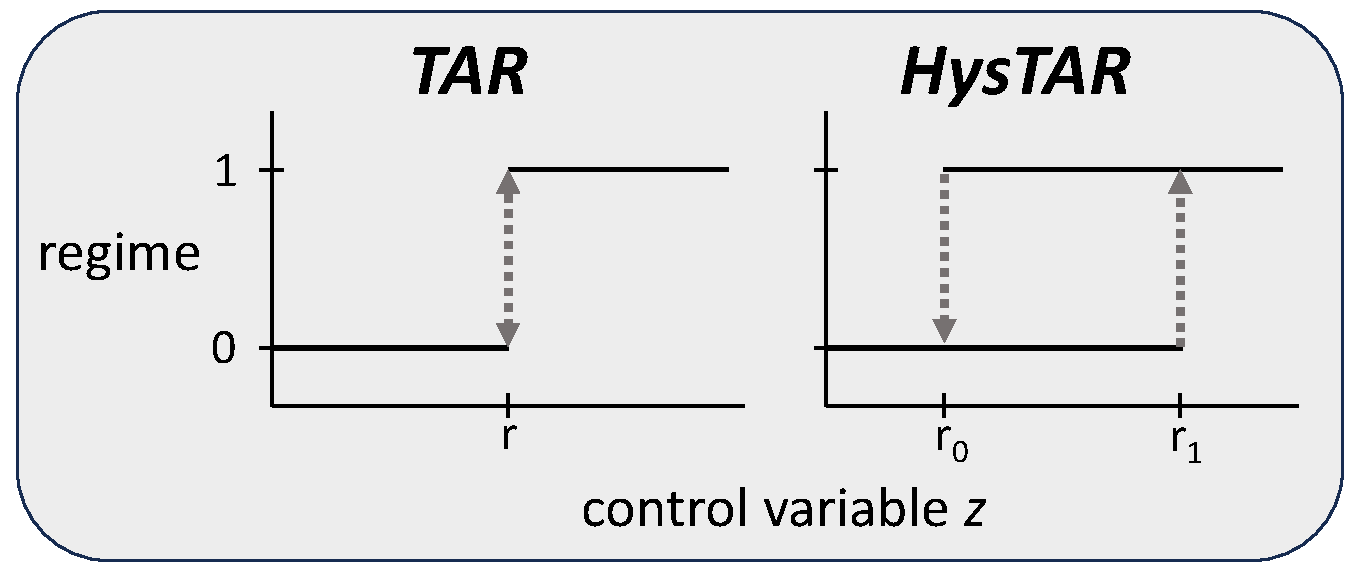
\includegraphics[scale=0.4]{simple_vs_hysteretic_2}
\caption{Regime switching in the TAR model (left) and in the HysTAR model (right). On the $y$-axis, we see the regimes, which can be 0 or 1. On the $x$-axis, we see the control variable. 
The black lines represents which regime is active for different levels of the control variable. The dotted arrows represent the sudden jumps between regimes.
For simple switches between regime 0 and 1, there is one threshold, $r$. For hysteretic switching, the switch from 0 to 1 has a threshold of $r_1$ and the switch from 1 to 0 has a threshold of $r_0$. Note that both regimes are possible when the control variable is between $r_0$ and $r_1$, which is called the hysteresis zone.}
\label{fig:simple_vs_hysteretic_2}
\end{figure}

The switches between regime 0 and 1 have the same threshold, regardless whether the switch is from regime 0 to 1 or from 1 to 0. 
This may not always be realistic: Sometimes, a switch from 0 to 1 cannot be reversed directly, because the control variable has to move to a different threshold  for a switch from 1 to 0.
For example, increasing external stress experienced by a person might push this person into a ``panick'' regime at a high stress level.
When the stress decreases again, it is plausible that it has to decrease to a much lower stress level to switch the regime back to ``relaxed''.
This phenomenon is called hysteresis.
To transfer the benefits of the TAR model into a model that can also account for hysteresis, \citet{bar2} proposed the hysteretic TAR model.

\subsection{HysTAR model}
In the hysteretic TAR model (HysTAR, also: buffered AR or hysteretic AR model), the dynamics of the outcome variable $y$ in each regime are modeled in the same way as in the TAR model (see Equation \ref{eqn:ar_processes}). The difference is in the regime switching equation, which can be expressed now as

\begin{equation} \label{eqn:hysteretic_switching}
R_t = \begin{cases}
0 & \mathrm{if} \, z_{t-d} \le r_0 \\
R_{t-1} & \mathrm{if} \, r_0 < z_{t-d} \le r_1 \\
1 & \mathrm{if} \, z_{t-d} > r_1. \\
\end{cases}
\end{equation}

In this equation, the regime $R_t$ remains unchanged when $z_{t-d}$ enters the \textit{hysteresis zone} $(r_0, r_1]$, which leads to the hysteresis effect. In the Figure \ref{fig:simple_vs_hysteretic_2}, it is illustrated how the HysTAR model differs from the TAR model.
That is, a switch from regime 0 to regime 1 happens when $z_{t-d}$ crosses $r_1$, but for a switch back from regime 1 to regime 0, $z_{t-d}$ has to cross the lower threshold $r_0$.
Note that the HysTAR model is equivalent to the TAR model if $r_0 = r_1$; hence, the TAR model is nested under the HysTAR model.

\section{Model estimation and inference}
\label{sec:LS_estimation}
We take it as a starting point that we already have established that there is threshold non-linearity in the observed data, for example by following the procedure proposed by \citet{testing_for_threshold_nonlinearity}, and now want to determine whether there is hysteresis in the mechanics underlying the regime switches.
Since the TAR model and HysTAR model only differ in the hysteresis effect, we can compare the model fit of the TAR model to the fit of the HysTAR model to detect hysteresis. This is described in Section \ref{sec:model_selection} and demonstrated in Section \ref{sec:simulation_study_1}.
But first, we providen some tools for parameter estimation and inference.

We implemented the least squares method proposed by \citet{bar2} to estimate the parameters of the HysTAR model in \textsf{R} \citep{R, R_hystar}, which we will briefly describe here.
For conciseness, we introduce the following notation.
Let $\phi = (\phi_{00}, \dots, \phi_{0 p_{0\max}}, \phi_{10}, \dots, \phi_{1 p_{1\max}})$ denote the  vector of AR coefficients, where $p_{0\max}$ and $p_{1\max}$ are the maximum orders we want to consider.
Let $d_{\max}$ denote the maximum delay we want to consider.
Let $r = (r_0, r_1)$ denote the vector of thresholds, where $r_0 \le r_1$.
Further, let $\sigma = (\sigma_{0}, \sigma_{1})$ denote the  vector of residual standard deviations.

For a given $p_0 \le p_{0\max}$ and $p_1 \le p_{1\max}$, our estimates of $\phi$, $r$, and $d$ are the values that minimize the sum of squared errors
\begin{equation} \label{eqn:sse}
L(\phi, r, d) := \sum_{t = k}^{T-1} (y_t - \hat{y}_t)^2,
\end{equation}

\noindent where
\begin{equation}
\hat{y}_t = 
\begin{cases}
\phi_{00} + \phi_{01} y_{t-1} + \cdots + \phi_{0 p_0} y_{t-p_0} 
& \text{if}~R_{t} = 0\\
\phi_{10} + \phi_{11} y_{t-1} + \cdots + \phi_{1 p_1} y_{t-p_1} 
& \text{if}~R_{t} = 1. \\
\end{cases}
\end{equation}

To select the appropriate orders $p_0$ and $p_1$, we cannot use least squares estimation, because the different orders have different numbers of $\phi$ parameters, and more $\phi$ parameters will always lead to lower values of $L(\phi, r, d)$. For this purpose, we use information criteria (Section \ref{sec:selecting_AR_orders}).
Also note that we start the summation of Equation \ref{eqn:sse} at $t = k :=\max\{d_{\max}, p_{0\max}, p_{1\max}\}$; the reason for this is that earlier observations cannot be modeled, because these would need lagged observations $y_{t-p_0}$, $y_{t-p_1}$, or $z_{t-d}$ that are unobserved.

\subsection{Parameter estimation} 
\label{sec:estimation}
Different values of the thresholds $r_0$ and $r_1$ can result in different assignments of the time points to the regimes. In turn, this leads to a different sum of squares. 
However, different regimes will only be assigned when $r_0$ or $r_1$ crossed an observed value of $z$. 
As a result, $L(\phi, r, d)$ is not continuous in $r$, so we cannot use the derivative to find the value of $r$ that minimizes the sum of squared errors.
This is solved by minimizing $L(\phi, r, d)$ over a discrete set. 
In the \texttt{hystar} package, this set consists of values that lie between the ordered observed values of $z$.
For example, when $z = (2, 4, 8, 6)$, these values are $\{3, 5, 7\}$.
Then, the search set of $\hat{r} = (\hat{r}_0, \hat{r}_1)$ would be $\{(3, 3), (3, 5), (3, 7), (5,5), (5, 7), (7, 7)\}$, since $\hat{r}_0 \le \hat{r}_1$ by design. Note that an estimate of 3 for $r_0$ is actually equivalent to all other values in the range $[2, 4]$ in this case.
In practice, often only the 80\% inner sample range of $z$ is used, to make sure that there are enough time points assigned to both regimes.

The sum of squared residuals is also not differentiable with respect to the delay parameter $d$, because $d$ takes on integer values. Therefore, the delay is optimized over the set $\{0, 1, \dots, d_{\max}\}$, where $d_{\max}$ is up to the researcher.

Fortunately, $L(\phi, r, d)$ is differentiable with respect to $\phi$ given $r$ and $d$. A closed form solution exists for the estimator $\hat{\phi}$ that minimizes the sum of squared errors (see Appendix \ref{app:estimation}). 
In this way, we can compute $\hat{\phi}$ for the finite combinations of $\hat{r}$ and $\hat{d}$, and select the solution that minimizes the sum of squared errors.

Finally, we can obtain estimates of the residual standard deviations in the following way. Denote the number of observations $k, \dots, T$ in regime $j$ by $n_j$. Then, the estimate of $\sigma_{j}$ is given by

\begin{equation}
\hat{\sigma}_{j} = \sqrt{\frac{1}{n_j} \sum_{t \in \{k, \dots, T-1\}| R_t = j} \big(y_t - \hat{y}_t \big)^2}.
\end{equation} 

\subsection{Estimation challenges}
Estimating the HysTAR model comes with two challenges that are not present in the standard TAR model.
First, the first regime $R_k$ may be undetermined for certain values of $\hat{r}$ and $\hat{d}$. 
This can be the case when the observation that determines the first regime, $z_{k-d}$, falls in the hysteresis zone.
A straightforward solution is to apply the estimation procedure to the cases where $y$ starts in regime 0 and where $y$ starts in regime 1, and choose the estimates with the smaller sum of squared errors.
However, when one of the AR orders is larger than the delay, there might be observations before $z_{k-d}$ that can inform us about the starting regime, if (one of) these are outside the hysteresis zone, see Figure \ref{fig:unknown_start}.

\begin{figure}
\begin{center}
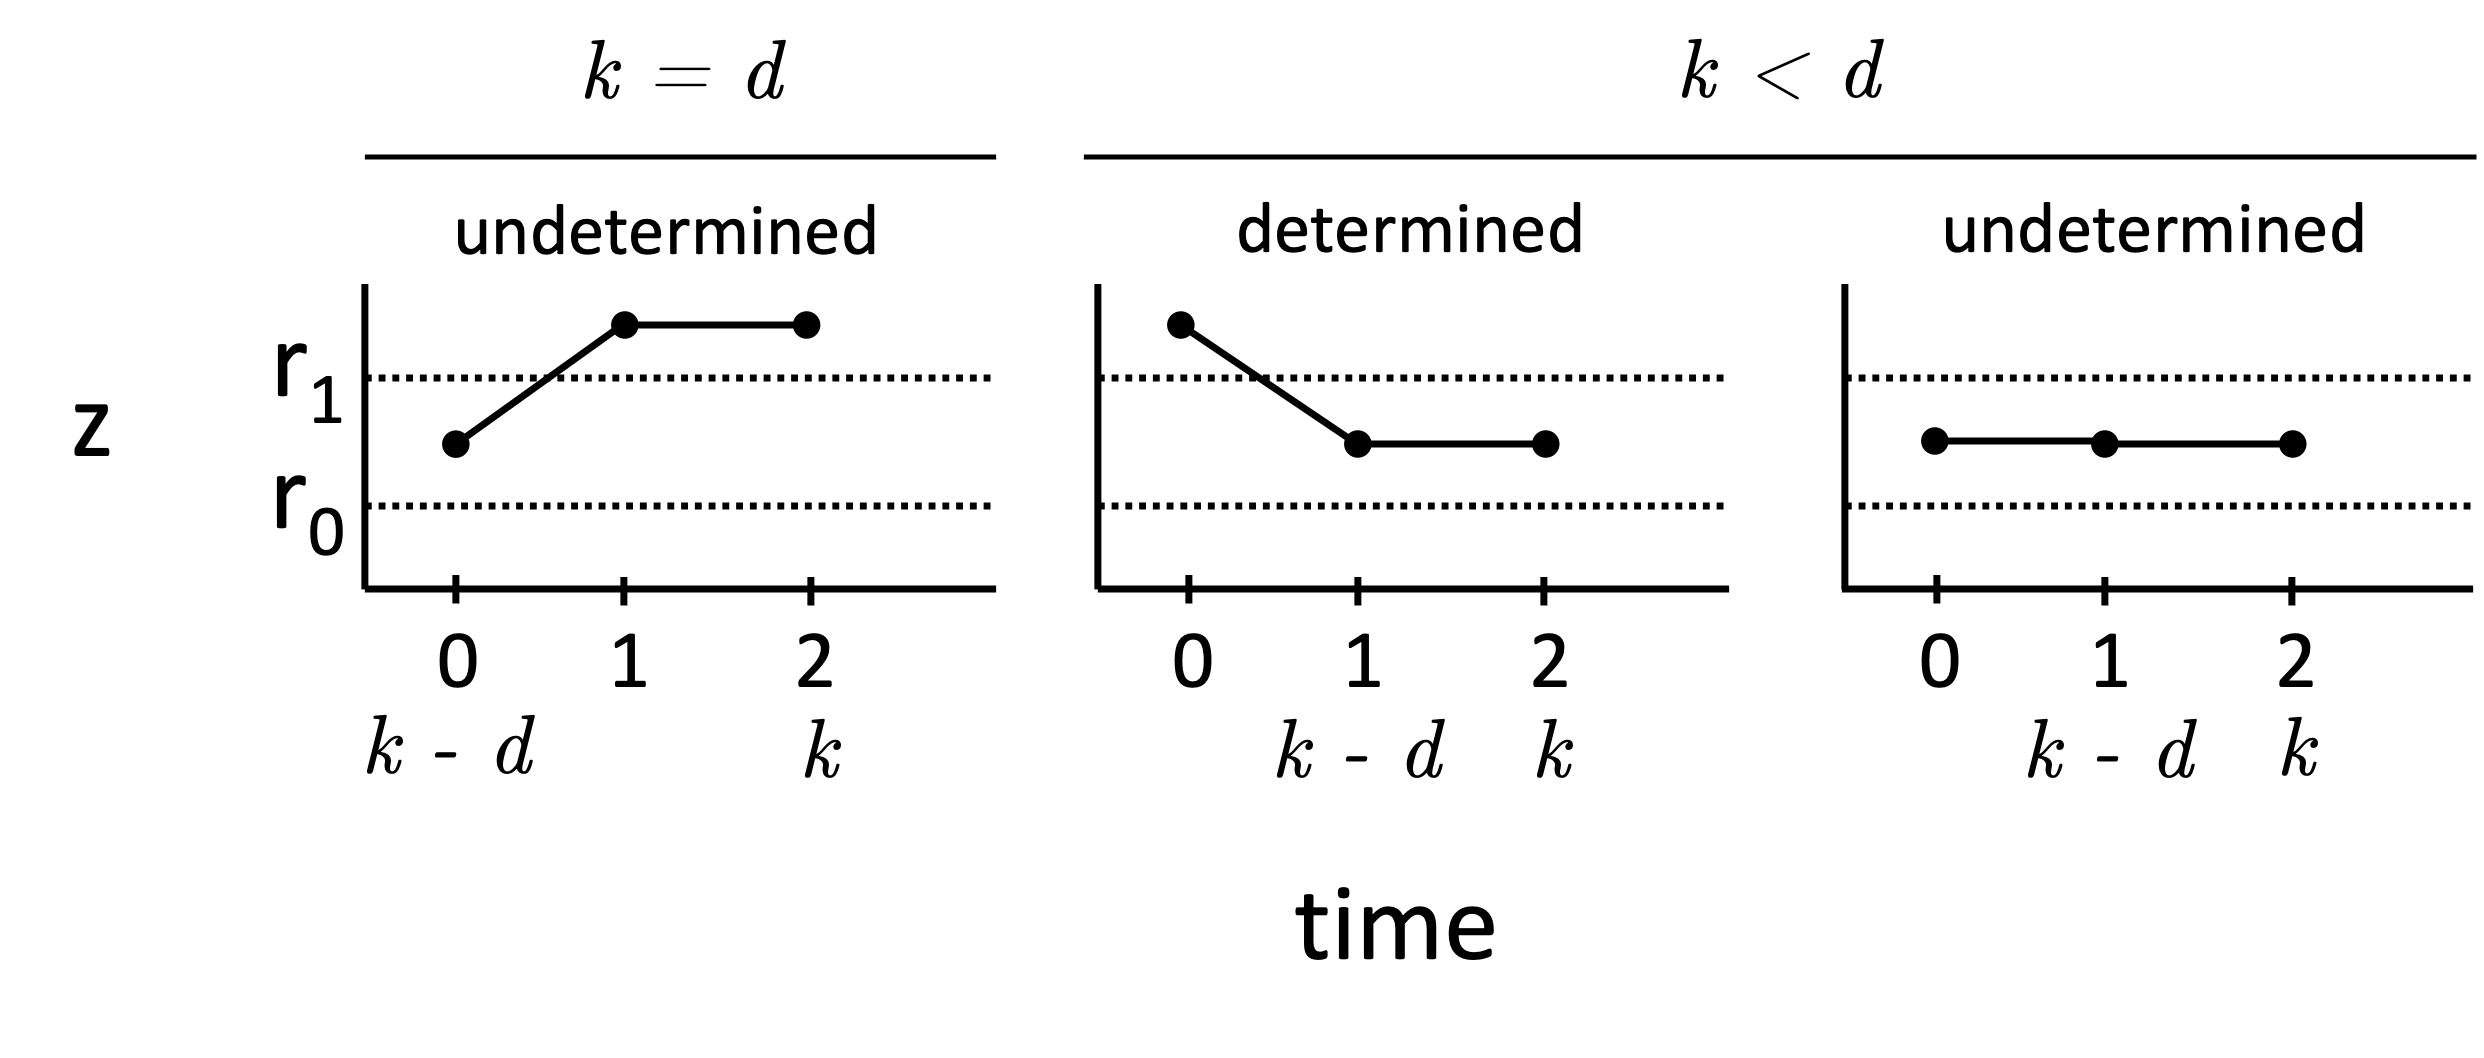
\includegraphics[scale=.6]{unknown_start.png}
\caption{\textit{Two situations where we want to determine the regime at time point $k$. 
If $k = d$, then $z_{k-d-1} = z_{-1}$ is unobserved. Hence, $R_{k-1}$ cannot be determined, so $R_{k}$ can also not be determined. We tackle this scenario by estimating the parameters twice, once while assigning $R_k = 0$, and a second time while assigning $R_k = 1$. Then, we choose the solution that yields the smallest sum of squared errors.
If $k > d$, we can have an interesting situation, since we have observations before $z_{k-d}$. 
Those observations $z_{0}, \dots, z_{k - d - 1}$ could be used to determine the regime at time point $k$, if at least one of them falls outside the hysteresis zone (see Figure \ref{fig:unknown_start}). This solution is implemented in the \texttt{hystar} package. 
However, if all $z_{0}, \dots, z_{k - d - 1}$ are in the hysteresis zone, we have to use the solution for the first scenario. (Note that $k < d$ is not possible by definition of $k$.)}}
\label{fig:unknown_start}
\end{center}
\end{figure}

Second, suppose we have two consecutive time points with the same regime, so $R_t = R_{t+1}$. This can result from two situations. First, $z_{t - d}$ and $z_{t - d + 1}$ are both outside the hysteresis zone, or second, $z_{t - d}$ is outside the hysteresis zone but $z_{t - d + 1}$ is inside the hysteresis zone. Both of these situations lead to the same sum of squared errors, because the series of regimes are exactly the same, but have different values for $r$.
In practice, we could choose the more conservative estimate (with the smallest hysteresis zone) and report equivalent estimates. Similarly, different estimates of $d$ can yield the same results (albeit with different threshold estimates associated with them). 
In that case, the convention is to choose the smallest $d$, which is more parsimonious \citep{bar2}, this is the default in the \texttt{hystar}-package.

\subsection{Parameter inference}
To draw conclusions about the parameter estimates, we need standard errors of the (asymptotic) sampling distributions of the estimators.
The estimator of the $\phi$-parameters are asymptotically normal \citep{bar2}, and we can obtain their standard errors analytically (see Appendix \ref{app:inference}).
The delay parameter $d$ is an integer, so $\hat{d}$ will equal $d$ when $T$ is large \citep{bar2}.
For the threshold parameters, however, we face a challenge, that is also known from threshold inference in the TAR model. 
The limiting distribution of $\hat{r}$ does not have a closed form and is very hard to approximate numerically \citep{bar2, li_least_2012}.
As a result, standard errors are not provided for $\hat{r}$ in the \texttt{hystar} package (these are also not provided for the \texttt{mTAR}-function to estimate the standard TAR model in the \textsf{R}-package \texttt{NTS} \citep{R_NTS}). 
To still gain some insight in how the threshold estimator behaves, we conducted a simulation study, which is described in Section \ref{sec:simulation_study_1}.

\subsection{Order selection}
\label{sec:selecting_AR_orders}
We can use information criteria to select the AR orders $p_0$ and $p_1$ (see \citet{information_criteria_tar} for an overview of information criteria in the context of threshold models). 
Then, we can select the orders that minimize the Akaike information criterion (AIC)

\begin{equation}
AIC(\hat{p}_0, \hat{p}_1) = \sum_{j = 0}^{1} \Big(n_j \log \hat{\sigma}_{j}^2 + 2(\hat{p}_j + 2) \Big),
\end{equation}

the corrected AIC (AICc)

\begin{equation}
AIC_c(\hat{p}_0, \hat{p}_1) = \sum_{j = 0}^{1} \Bigg( n_j \log \hat{\sigma}_{j}^2 + 
\frac{2(\hat{p}_j + 2)}{n_j - \hat{p}_j - 3} \Bigg)
\end{equation}

or the Bayesian information criterion (BIC)

\begin{equation}
BIC(\hat{p}_0, \hat{p}_1) = \sum_{j = 0}^{1} \Big( n_j \log \hat{\sigma}_{j}^2 + (\hat{p}_j + 2)  \log n_j \Big).
\end{equation}

Note that we use $\hat{p}_j + 2$ for the number of parameters within a regime, namely $\hat{p}_j$ autoregressive effects, one intercept and a residual standard deviation.

\subsection{Model selection} \label{sec:model_selection}
Since the standard error of the threshold estimator is unknown, it cannot be used to choose between the TAR model and the HysTAR model.
Otherwise, overlapping confidence intervals for the estimates of $r_0$ and $r_1$ could indicate a preference for the TAR model, where $r_0$ and $r_1$ are equal.
Unfortunately, we can also not use a likelihood-ratio test to compare the HysTAR to the TAR model (G. Li, personal communication, June 1, 2023).
So, we need an alternative approach to assess whether hysteresis is present in the dynamics of the system under investigation.

In the current paper, we propose to estimate information criteria for both models, and select the model with smaller values.
Note that the information criteria presented in Section \ref{sec:selecting_AR_orders} do not penalize the threshold parameter(s), and that the HysTAR model has one threshold parameter more than the TAR model.
Ignoring this difference may lead to overfitting of the HysTAR model.
Therefore, we adopt an AIC-type information criterion developed for change point models \citep[AICcp][]{aiccp}, where the penalty of a threshold parameter is 6, that is,

\begin{equation}
\label{eq:aiccp}
AIC_{CP} = \sum_{j = 0}^{1} \Big(n_j \log \hat{\sigma}_{j}^2 + 2(\hat{p}_j + 2) \Big) + 6a,
\end{equation}

\noindent where $a$ is the number of thresholds.

Additionally, we can assess whether the residuals of the model follow a white noise process, which should be the case according to both models.
Since the observations of a white noise process are all uncorrelated with each other, we can check whether the autocorrelations of the residuals are not significantly different from zero.
This can be done at once with the Ljung-Box test, for example, that tests the null-hypothesis that the autocorrelations are zero \citep{ljungbox}, but also by visualizing the autocorrelation function (ACF) of the residuals.
We assess the performance of the model selection methods presented here in a simulation study 1 (Section \ref{sec:simulation_study_1}).

\section{Simulation study 1: Model selection}
\label{sec:simulation_study_1}
Detecting hysteresis in empirical time series data raises several practical questions.
For example, does it matter how many regime switches have taken place?
Does it matter how the regimes differ from each other?
And how large does the hysteresis zone need to be?
These questions are addressed in simulation study 1.

\subsection{Simulation setup}
In simulation study 1, we considered the following conditions: 50, 100, 200 and 400 time points, 2, 5, and 10 regime switches (denoted by $N_{\mathrm{rs}}$), (un)equal means and (un)equal autoregression between the regimes, and hysteresis zones $(0, 0]$, $(-0.25, 0.25]$ and $(-0.5, 0.5]$. For each condition, we generated 500 replications of time series of the control variable $z$ and the outcome variable $y$ from the HysTAR model.

This results in a total of $4 \times 3 \times 3 \times 3 = 108$ conditions.
To obtain the differences in regimes in means and autoregression, we use $\phi = (\phi_{00}, \phi_{01}, \phi_{10}, \phi_{11}) = (0, 0.6, 0, 0.2)$, $(0, 0.6, 3, 0.2)$ and $(0, 0.4, 3, 0.4)$. Note that the means of regime $j$ is given by $\phi_{j0}/(1 - \phi_{0j})$.
In all conditions, we set the delay parameter to $d = 0$ and use equal residual variances in the regimes, $\sigma_0^2 = \sigma_1^2 = 1$. 
Furthermore, to control the number of regime switches, the time series of the control variable is a sine wave, going up and down between $-1$ and $1$ the desired number of times.
Since hysteresis zones are centered around zero in the current setup, this results in an equal amount of observations in both regimes for 2 and 10 switches, and slightly more observations in regime 0 when there are 5 regime switches.
In Figure \ref{fig:ts_examples}, we give three examples of time series generated from the HysTAR model.

\begin{figure} 
\caption{Examples of generated data from the HysTAR model}
\begin{center}
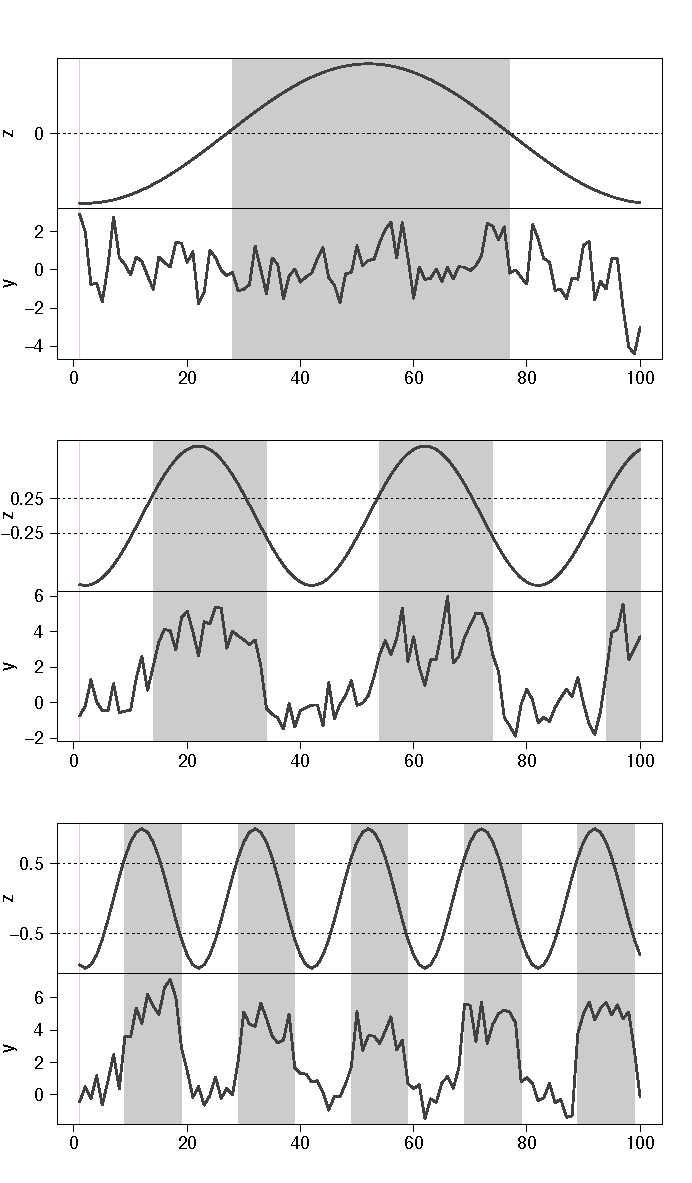
\includegraphics[scale=.6]{ts_examples}
\end{center}
\bigskip
\small\textit{Note}. Each of the examples have a different number of regime switches, a different hysteresis zone and a different difference between the regimes, from top to bottom: 1) 2 switches, $r = (0, 0]$, equal mean - unequal autoregression. 2) 5 switches, $r = (-0.25, 0.25]$, unequal mean - unequal autoregression. 3) 10 switches, $r = (-0.5, 0.5]$, unequal mean - equal autoregression. For all examples, $T = 100$. Plots were generated with the \texttt{hystar} package in \textsf{R}, and code to create the plots can be found in the supplementary material.
\label{fig:ts_examples}
\end{figure}

To see whether we can detect the hysteresis effect, we fit the HysTAR model and TAR model to each data set within a condition.
The AIC, BIC, AICc AICcp are used to select the HysTAR or TAR model, by choosing the model with the smaller value.
In case of equal values for an information criterion, we select the TAR model, because it is more parsimonious (this will happen when the HysTAR threshold estimates are equal, which is not unlikely when the TAR model is the true model). 
Additionally, we conduct the Ljung-Box test on the residuals of both models, to test the hypotheses that the residuals are uncorrelated.
A significant result from the Ljung-Box test implies that the residuals are correlated, and hence, a model does not capture the dependencies in the data well.
We select a model when the $p$-value of its Ljung-Box test is non-significant ($>0.05$) and for the other model it is significant. Otherwise, the choice remains undecided.

In fitting the models, we assume the orders of the regimes known, because we want to focus on model selection between the HysTAR and the TAR model rather than order selection, which is also typically done by comparing information criteria. 
We also assume the delay parameter known. 
In our simulations, the HysTAR model is equivalent to a TAR model with very large delay, since the the control variable moves symetrically around the hysteresis zone.
Therefore, fixing the delay parameter to zero will lead to a clear distinction between the HysTAR and TAR model.
Of course, this is not needed in practice, where $z$ will behave less predictable and the thresholds are not always exactly located around the median of $z$.

\subsection{Results}
\label{sec:model_selection_results}
The code to reproduce this simulation study can be found in the online supplementary materials.
\footnote{\url{https://github.com/daandejongen/hysteresis_paper}}
In Table \ref{tab:model_selection_results}, we present the proportion of correctly selected models according to the BIC and AICcp within each condition. Results of the AIC and AICc are omitted here, because their values are very similar to the BIC. In general, we see that information criteria can detect hysteresis if the regimes have different means and $T$ is sufficiently large. 
The Ljung-Box test was not able to detect the HysTAR model very well. However, the test has a very high \textit{precision} (also: positive predictive value), for many conditions 100\%. So when there is hysteresis, comparing the Ljung-Box results does not indicate hysteresis very often. But when the Ljung-Box comparison is positive, hysteresis is nearly always present.
Its results are provided in the supplementary material, as well as 

When we compare the BIC to the AICcp, we see that the AICcp performs better when the data are generated from a TAR model, and the BIC performs better when the data are generated from HysTAR model. This is unsurprising at first glance, since the AICcp penalizes the HysTAR model 6 points harder than the TAR model. Interestingly, it does not seem to matter much how large the hysteresis zone is, when the HysTAR is the true model.
	This difference between the BIC and AICcp is especially pronounced in the case where the regimes have the same mean. Apparently, the BIC value of the HysTAR model is only slightly higher than that of the TAR model in this case, such that the threshold penalty in the AICcp leads to a preference for TAR model. However, regardless of whether the correct type of model is selected or not in this case, the results in simulation study 2 (\ref{sec:simulation_study_2}) show that the estimators of the thresholds have very large bias and variance. Hence, results from both models are hard to interpret.
	When the regimes do not have the same mean, they are much more easily disentangled. For $T\ge 200$, we see that both information criteria perform very well, although the BIC still performs not so well when the TAR model is true.

When the number of regime switches $N_{\mathrm{rs}}$ increases, model selection becomes better when the true model is a TAR, but worse when the true model is a HysTAR. 
This seems interesting, but we suspect that this an artifact from the way the control variable was simulated, as more switches leads to fewer unique values in $z$ (denoted by \#$z$). In turn, this leads to a higher possibility that $r_0$ and $r_1$ have the same estimate, such that a TAR model is chosen.
This makes it hard to disentangle the effects of $T$, $N_{\mathrm{rs}}$ and \#$z$.
However, we can see that \#$z$ is not the only important variable.
For example, when comparing conditions with equal \#$z$, for example $T = 200$, $N_{\mathrm{rs}} = 5$ with $T = 400$, $N_{\mathrm{rs}} = 10$, model selection is better in the second case.
So, there is still additional value to higher $T$ or $N_{\mathrm{rs}}$.
Furthermore, the $z$-values themselves play an imporant role. 
In the case with $r = (-0.25, 0.25]$, $T = 50$ and $N_{\mathrm{rs}} = 10$, the observed $z$-values are not close to the true threshold, leading to very poor performance of the information criteria.
Therefore, it is important to observe enough $z$-values around the true threshold.

\subsection{Conclusion}
To detect hysteresis in a regime switching process, comparing information criteria can be a viable method, that compensate for the unavailability of direct statistical hypothesis tests. However, this only holds when the regimes differ in mean, in which case the change point AIC performs best. For regimes with equal means, the best performing information criterion depends on whether there is hysteresis or not in the data generating mechanism, which is the research question in the first place. The Ljung-Box test seems be too conservative to detect the correlations in wrongly specified models.

% latex table generated in R 4.2.1 by xtable 1.8-4 package
% Fri Nov 17 11:19:39 2023
\begin{table}
\caption{Proportion correct model selection according to the BIC and AICcp}
\begin{tabular}{rrr cc cc cc}
\hline
$T$ & $N_{\mathrm{rs}}$ & \#$z$ & \multicolumn{2}{c}{eq.-uneq.} & \multicolumn{2}{c}{uneq.-uneq.} & \multicolumn{2}{c}{uneq.-eq.} \\
\cline{4-9}
\multicolumn{3}{l}{} & BIC & AICcp & BIC & AICcp & BIC & AICcp \\
\hline
  \multicolumn{9}{c}{$r = (0, 0]$ (TAR model)} \\
  50  & 2  & 19  & 0.39 & 0.94 & 0.64 & 0.95 & 0.84 & 0.99 \\ 
  50  & 5  & 8   & 0.51 & 0.97 & 0.80 & 0.98 & 0.98 & 0.99 \\ 
  50  & 10 & 3   & 0.71 & 0.99 & 0.95 & 1.00 & 1.00 & 1.00 \\ 
  100 & 2  & 40  & 0.29 & 0.95 & 0.63 & 0.96 & 0.86 & 0.99 \\ 
  100 & 5  & 16  & 0.39 & 0.96 & 0.80 & 0.98 & 0.97 & 1.00 \\ 
  100 & 10 & 8   & 0.53 & 0.96 & 0.95 & 0.99 & 1.00 & 1.00 \\ 
  200 & 2  & 80  & 0.26 & 0.93 & 0.63 & 0.98 & 0.87 & 0.99 \\ 
  200 & 5  & 32  & 0.33 & 0.94 & 0.81 & 0.98 & 0.98 & 1.00 \\ 
  200 & 10 & 16  & 0.42 & 0.97 & 0.95 & 0.99 & 1.00 & 1.00 \\ 
  400 & 2  & 160 & 0.26 & 0.96 & 0.66 & 0.96 & 0.86 & 0.99 \\ 
  400 & 5  & 64  & 0.28 & 0.96 & 0.85 & 1.00 & 0.98 & 1.00 \\ 
  400 & 10 & 32  & 0.39 & 0.97 & 0.96 & 1.00 & 1.00 & 1.00 \\
  \hline
  \multicolumn{9}{c}{$r = (-0.25, 0.25]$ } \\
  50  & 2  & 19  & 0.65 & 0.06 & 0.97 & 0.60 & 0.98 & 0.88 \\ 
  50  & 5  & 8   & 0.52 & 0.04 & 0.81 & 0.37 & 0.95 & 0.74 \\ 
  50  & 10 & 3   & 0.30 & 0.01 & 0.05 & 0.01 & 0.00 & 0.00 \\
  100 & 2  & 40  & 0.76 & 0.10 & 1.00 & 0.93 & 1.00 & 0.99 \\ 
  100 & 5  & 16  & 0.65 & 0.09 & 0.98 & 0.80 & 1.00 & 0.99 \\ 
  100 & 10 & 8   & 0.57 & 0.06 & 0.92 & 0.69 & 1.00 & 0.98 \\ 
  200 & 2  & 80  & 0.86 & 0.14 & 1.00 & 1.00 & 1.00 & 1.00 \\ 
  200 & 5  & 32  & 0.76 & 0.11 & 1.00 & 0.99 & 1.00 & 1.00 \\ 
  200 & 10 & 16  & 0.71 & 0.10 & 1.00 & 0.98 & 1.00 & 1.00 \\ 
  400 & 2  & 160 & 0.93 & 0.32 & 1.00 & 1.00 & 1.00 & 1.00 \\ 
  400 & 5  & 64  & 0.91 & 0.32 & 1.00 & 1.00 & 1.00 & 1.00 \\ 
  400 & 10 & 32  & 0.88 & 0.32 & 1.00 & 1.00 & 1.00 & 1.00 \\ 
  \hline
  \multicolumn{9}{c}{$r = (-0.5, 0.5]$ } \\
  50  & 2  & 19  & 0.64 & 0.08 & 0.99 & 0.86 & 1.00 & 0.95 \\ 
  50  & 5  & 8   & 0.56 & 0.05 & 0.98 & 0.77 & 1.00 & 0.97 \\ 
  50  & 10 & 3   & 0.46 & 0.05 & 0.98 & 0.89 & 1.00 & 0.99 \\
  100 & 2  & 40  & 0.77 & 0.16 & 1.00 & 0.99 & 1.00 & 1.00 \\ 
  100 & 5  & 16  & 0.74 & 0.15 & 1.00 & 0.98 & 1.00 & 1.00 \\ 
  100 & 10 & 8   & 0.61 & 0.10 & 1.00 & 0.98 & 1.00 & 1.00 \\ 
  200 & 2  & 80  & 0.88 & 0.29 & 1.00 & 1.00 & 1.00 & 1.00 \\ 
  200 & 5  & 32  & 0.84 & 0.24 & 1.00 & 1.00 & 1.00 & 1.00 \\ 
  200 & 10 & 16  & 0.87 & 0.33 & 1.00 & 1.00 & 1.00 & 1.00 \\ 
  400 & 2  & 160 & 0.94 & 0.57 & 1.00 & 1.00 & 1.00 & 1.00 \\ 
  400 & 5  & 64  & 0.96 & 0.57 & 1.00 & 1.00 & 1.00 & 1.00 \\ 
  400 & 10 & 32  & 0.93 & 0.58 & 1.00 & 1.00 & 1.00 & 1.00 \\ 
   \hline
\end{tabular}
\newline
\small\textit{Note}.
$T$ = number of time points,
$N_{\mathrm{rs}}$ = number of regime switches,
\#$z$ = number of unique values in the 80\% inner range of $z$.
(un)eq.-(un)eq. = (un)equal means-(un)equal autoregression.
BIC = Bayesian information criterion, AICcp = change point Akaike information criterion.
$r$ is the hysteresis zone.
\label{tab:model_selection_results}
\end{table}



\section{Simulation Study 2: Parameter estimation}
\label{sec:simulation_study_2}
Although the asymptotic distribution of $\hat{\phi}$ is known, we don't know how well it performs in finite samples.
For the threshold estimator, it is even more important to assess its finite sample performance.
In simulation study 2, we investigate how well the parameters of the HysTAR model can be recovered. That is, we estimate the HysTAR model with data generated from the HysTAR model and assess how close the parameter estimates are to the true parameter values.
For this study, we use the exact same generated data sets as in simulation study 1.

\subsection{Performance measures}
Unbiasedness, efficiency and consistency are well-known desirable properties of estimators. Therefore, within each condition, we compute the empirical bias $N_R^{-1} \sum (\hat{\theta} - \theta)$, the empirical variance $N_R^{-1} \sum (\hat{\theta} - \bar{\theta})^2$ and the mean squared error $N_R^{-1} \sum (\hat{\theta} - \theta)^2$, where the summation is over the $N_R$ replications in a condition, $\hat{\theta}$ is an estimate of the parameter $\theta$ and $\bar{\theta}$ denotes the mean of the estimates.
For an unbiased estimator, the bias is zero.
An efficient estimator has low variance and a consistent estimator is unbiased and has a variance that approaches zero as $T \rightarrow \infty$.
These properties are assessed visually.
Note that the estimator of $\phi$ is known to be asymptotically unbiased and consistent, so we should see a bias and a variance that approach zero as $T$ increases.

We also check coverage rates of the confidence intervals, that is, the proportion of times the estimated 95\% confidence interval of a $\phi$-parameter contains the true value of that $\phi$-parameter, which should be 95\%. Additionally, the mean of the estimated standard errors of a parameter should be close to the empirical standard deviation of the estimates of that parameter.

\begin{figure}
\caption{Empirical bias and variance of $\hat{r}_0$ (top pane) and $\hat{r}_1$ (bottom pane)}
\begin{center}
\makebox[0pt]{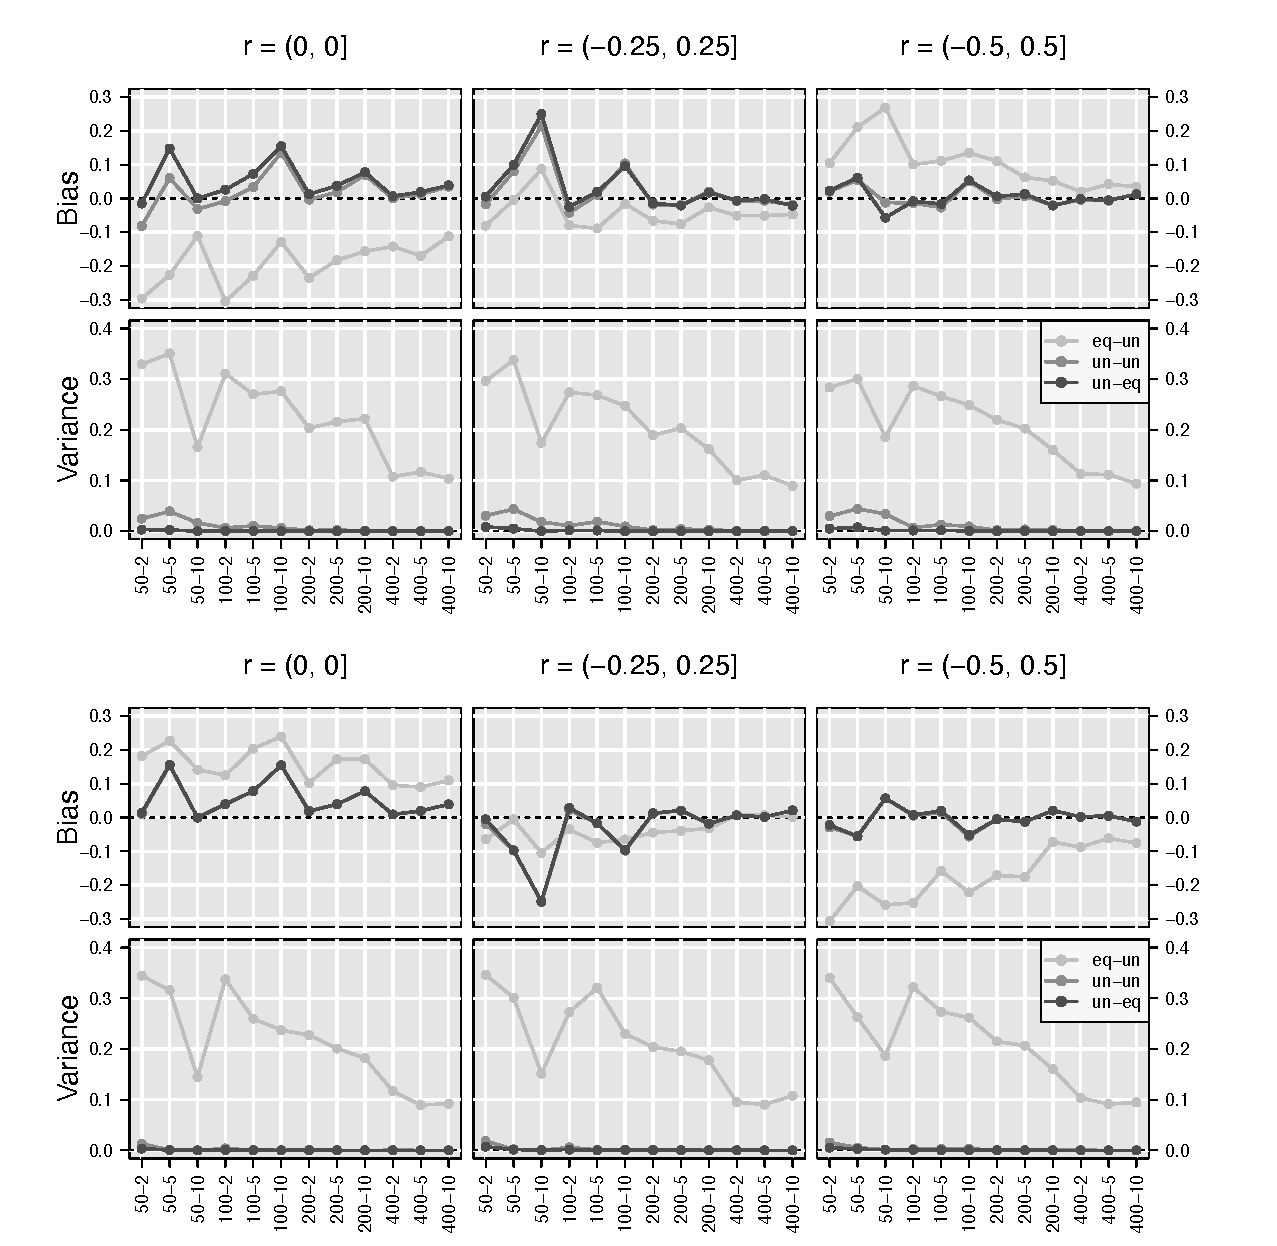
\includegraphics[scale=.75]{simulation_results_r0_r1}}
\end{center}
\bigskip
\textit{Note}. (un)eq-(un)eq = (un)equal means-(un)equal autoregression. The bias is $N_R^{-1} \sum (\hat{r}_j - r_j)$ and the variance is $N_R^{-1} \sum (\hat{r}_j - \bar{r}_j)^2$, where the number of replications $N_R$ in each condition is 500, $\bar{r}_j$ denotes the mean of the estimates and $j \in \{0, 1\}$ denotes the regime. Code to reproduce this plot can be found in the supplementary materials.
\label{fig:simulation_study_2_results}
\end{figure}

\subsection{Results}
In Figure \ref{fig:simulation_study_2_results}, the bias and variance of the threshold estimators are presented.
Results for the $\phi$-parameters are omitted here, since all estimators clearly show the disired properties, apart from $\hat{\phi}_{10}$, that converges somewhat slower than the other $\phi$-parameters. 
All results not presented here can be found in the supplementary material, as well as the code to reproduce this simulation study.

In general, the threshold estimators seem to be consistent, because the variances converge to zero when $T$ increases, which is in line with the analytical results of \cite{bar2}.
However, we also need to consider the bias, which is not always zero. 
With equal means and $r = (0, 0]$, $\hat{r}_0$ has negative bias and $\hat{r}_1$ positive bias, which seems intuitive since $\hat{r}_0 \le \hat{r}_1$ by design, so the true value is at the boundary of the search space.
For equal means and $r = (-0.5, 0.5]$, we see quite the opposite, and both estimators are negatively biased for equal regime means and $r = (-0.25, 0.25]$. However, with such large variances (for equal means), differences in bias may be less important.

When the regimes have equal means, we see different patterns for the bias. For $r = (0, 0]$, the threshold estimators follow a similar positive pattern, which is quite  interesting, since there seems to be no clear explanation for that.
A ``mirroring'' pattern around zero can be seen for $r = (-0.25, 0.25]$ or $r = (-0.5, 0.5]$. Here, the estimates are conservative, that is, the hysteresis zone is often underestimated.
However, for $T\ge 200$, the bias becomes almost negligible.
Also interesting is the fact that for the estimation of $r_1$, an euqal or unequal autoregressive parameter does not seem to make any difference at all.

The variance of the estimators show that the model has difficulty recognizing the threshold when the regimes have equal means, which was also clear from the model selection results in Section \ref{sec:model_selection_results}. 
Also in line with the previous section is the dip in variance for $T = 50$ and $N_{rs}= 10$, resulting directly from the small number of possible estimates in this case.
When the regimes have equal means, the variances of the estimators are very low, which is, of course, only desirable when the bias is also low.

We note two more observations about estimation of the thresholds. 
First, when the autoregression in regime 0 is larger than in regime 1, a regime switch from 1 to 0 (caused by threshold $r_0$) will be ``slower'' than a switch from 0 to 1. That is, it takes longer to arrive at the mean of regime 1, because of the larger autoregression. 
As a result, the first few observations in regime 0 will also fit well in regime 1. Therefore, estimation of $r_0$ will be harder than estimation of $r_1$. 
This is reflected by the fact that the variance of $\hat{r}_0$ is somewhat larger than the variance of $\hat{r}_1$ when the regimes have unequal autoregression, and is most visible for low $T$.
Second, we can see small peaks in the variances where $N_{rs} = 5$ for $\hat{r}_0$, and not for $\hat{r}_1$. 
When $N_{rs} = 5$, there will be 3 switches caused by $r_1$ and 2 switches by $r_0$, because the generated data always start in regime 0. As a result, $r_1$ is easier to estimate, in that case.

\section{Empirical example 1: Depression} 
\label{sec:empirical_example_1}
In the first simulation study, the data generating mechanism was the HysTAR model. 
Of course, there exist other models that produce the hysteresis effect.
Therefore, in the second simulation study, we generate data from a different mechanism that gives rise to hysteretic regime-switching, which should still be picked up by the HysTAR model.

One research area where there has been particular interest in the phenomenon of hysteresis is the network approach to psychopathology \citep{borsboom_psychometric_2008}.
We follow an example of a network model of major depression as studied by \citet{cramer_major_2016}.
This network consist of 14 connected depression symptoms that can be switched on or off, where the sum of symptoms that are switched on is the level of depression.
The symptoms trigger their neighboring symptoms to switch on or off, over time. For example, fatigue may lead to depressed mood, which in turn leads to loss of interest, which again leads to fatigue, et cetera.
With the existence of such feedback loops, two stable regimes can emerge: one where most symptoms are switched on, representing a depression, and one where most symtoms are switched off, representing a healthy regime.

Depression networks in which the symptoms are highly connected are said to be vulnarable to external stress.
That is, when external stress triggers a symptom to switch on, this will  quickly result in a ``cascade'' of symptoms switching on.
In the study by \citet{cramer_major_2016}, external stress triggering the symptoms was simulated to go up an down over time.
In this way, stress is a control variable that causes switches between the healthy and depressed regime.
The authors found support for a hysteresis effect in these switches by fitting the cusp catastrophe model with the \texttt{cusp} package in \textsf{R} \citep{R, R_cusp}.

In the current study, we replicated the simulation by \citet{cramer_major_2016} with 1000 time points. 
We used the same network (same nodes and connections), which was based on empirical data \citep{network_data}. 
The stress levels were varied between -1 and 1. 
We estimated the HysTAR model with $d_{\max} = 1$, $p_0 = p_1 = 1$  and a threshold search space in the 80\% inner sample range of stress, which were stress levels between -0.947 and 0.947.
The $\mathsf{R}$-code that was used to run the simulation can be found in the supplementary materials.

\subsubsection{Results}
Figure \ref{fig:ts_plot_MD} shows the simulated time series of stress and depression.
In Table \ref{tab:results_MD}, the HysTAR and TAR model estimates are shown.
According to the AIC, AICc and BIC, the HysTAR model is preferable.
The Ljung-Box results were indecisive, in the sense that these indicated that both models fit well.
The autocorrelations of the residuals are presented in Figure \ref{fig:resplot_MD} and indicate a preference for the HysTAR model, since the TAR model has a significant autocorrelation at lag 1.
The difference between the threshold estimates indicates a substantial hysteresis effect, $\hat{r}_1 - \hat{r}_0 = 0.55 - (-0.33) = 0.88$.
Additionally, the $\phi$ parameters show a clear distinction between the regimes. The mean depression score as implied by the AR coefficients is 0.85 regime 0 and 9.09 in regime 1,
such that we can interpret regime 0 as the healthy regime and regime 1 as the depression regime. We also see that the depression regime has a stronger autoregression, which is supported by empirical evidence \citep{kuppens_emotional_2010, koval_getting_2012}.
Notably, these dynamic differences were not found in the original study by \citet{cramer_major_2016}, because the cusp catastrophe model does not allow for dynamic differences between regimes.

\begin{figure} 
\begin{center}
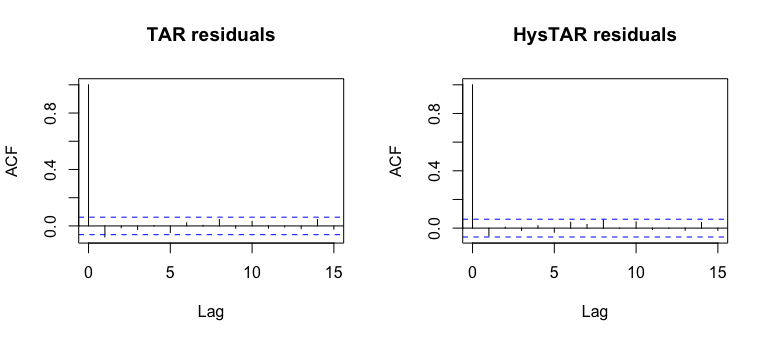
\includegraphics[scale=.6]{resplot_MD_both}
\caption{\textit{Autocorrelation function estimates for the residuals of the TAR model and the HysTAR model. The dashed lines represent the 95\% confidence interval around 0.}}
\label{fig:resplot_MD}
\end{center}
\end{figure}

\begin{figure} 
\begin{center}
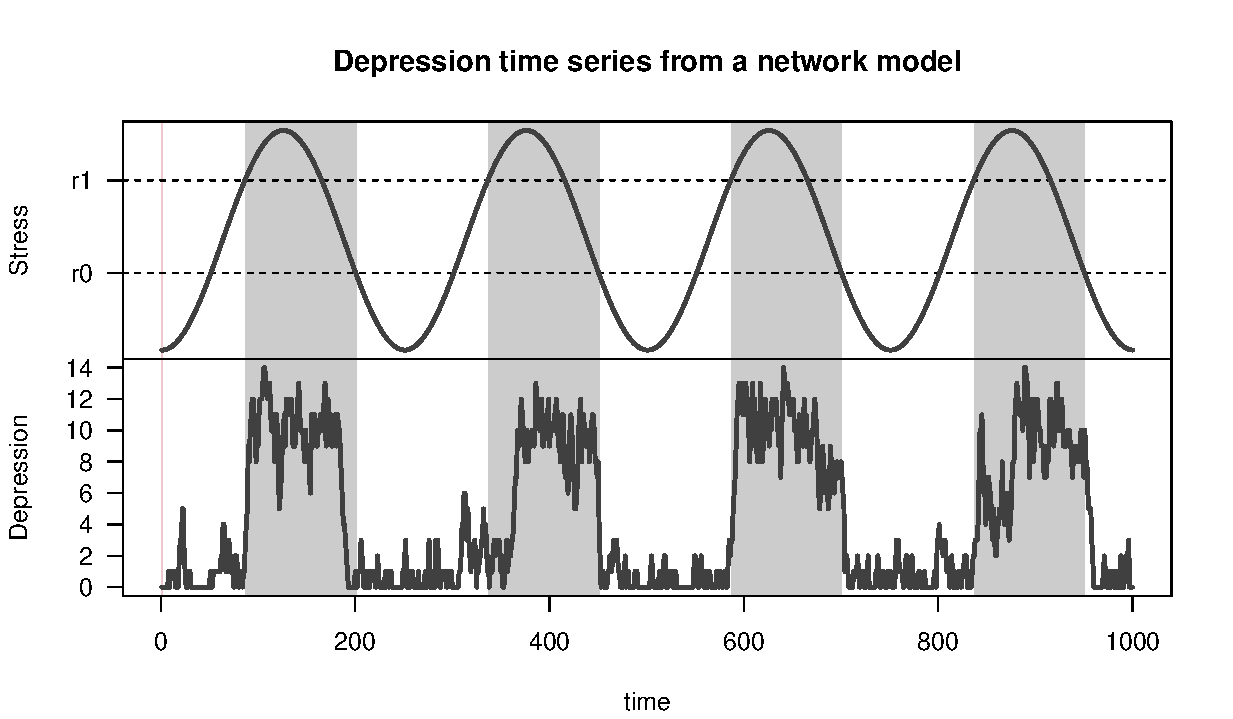
\includegraphics[scale=.6]{ts_plot_MD}
\caption{\textit{Time series plots of stress and depression, simulated from a network model. The dashed lines represent the estimates threshold values of the HysTAR model. The grey background represents the depressed regime and the white background represents the healthy regime.}}
\label{fig:ts_plot_MD}
\end{center}
\end{figure}

\begin{table}[h!]
\begin{center}
\begin{tabular}{ c c c c c }
\hline
 & \multicolumn{2}{c}{HysTAR} & \multicolumn{2}{c}{TAR} \\
 \hline
Parameter & Est. & 95\% CI & Est. & 95\% CI \\
\hline
$\phi_{00}$ & 0.23 & $[0.14, 0.31]$ & 0.206 & $[0.12, 0.29]$ \\
$\phi_{01}$ & 0.73 & $[0.68, 0.78]$ & 0.677 & $[0.62, 0.73]$ \\
$\phi_{10}$ & 1.00 & $[0.64, 1.36]$ & 0.414 & $[0.21, 0.62]$ \\
$\phi_{11}$ & 0.89 & $[0.85, 0.93]$ & 0.944 & $[0.92, 0.97]$ \\
$r_0$ & -0.30 & - & -0.30 & - \\
$r_1$ & 0.55 & - & -0.30 & - \\
$d$ & 0 & - & 1 & - \\
$\sigma_0$ & 0.70 & - & 0.58 & - \\
$\sigma_1$ & 1.93 & - & 1.79 & - \\
\multicolumn{5}{c}{Information criteria} \\
\hline
AIC  & 116.19 & - & 136.59 & - \\
AICc & 116.28 & - & 136.69 & - \\
BIC  & 141.44 & - & 161.76 & - \\
AICcp & 128.19 & - & 142.59 & - \\
\hline
\end{tabular}
\caption{Parameter estimates of the HysTAR model and TAR model on data simulated from an empirical depression model, $T = 1000$.}
\label{tab:results_MD}
\end{center}
\end{table}

\section{Empirical example 2: Speed-accuracy Trade-off} \label{sec:empirical_example_2}
The HysTAR model has been succesfully applied to economic time series, such as growth rates of stocks and prices \citep{tsay}, daily number of stock trades \citep{liu}, air pollution \citep{chen} and quarterly GDP growth \citep{bar2}. However, the HysTAR model has not been used to investigate hysteresis in psychological processes, so far.

Therefore, we reanalyzed data from the speed-accuracy trade-off experiment by \citet[][experiment 1b]{speedaccuracy}, with the HysTAR model, which were originally analyzed with a hidden Markov model.
In this hidden Markov model, hysteretic switches can be inferred from time series data, but the dynamics within regimes are not modeled.
We selected participants F and I, corresponding to the participant labels used in the original study, because these participants showed clear hysteresis effects.
Participant F performed a lexical decision task where they had to discriminate word from non-word stimuli and participant I had to judge whether a horizontal line crossing a vertical line extended more to the right or to the left.
The researchers measured the response time (RT) and response accuracy (RA) of the participants.
For each response, the participants received a payoff for speed and a payoff for accuracy, always summing op to 24 units of total payoff.
When participants receive 24 units for a fast answer (so zero for an accurate answer), we expect them to behave according to a guess (G) regime with low response time and low accuracy.
On the other hand, if there is only payoff for accurate answers, participants will follow a stimulus-controlled (SC) regime with high response time and high accuracy.
The focus in the study was on the transitions between the two regimes under gradual changes of payoff for accuracy $P^{\mathrm{AC}}_t$, which was under the control of the researchers.
The researchers expected that the regime switches would happen at different values of $P^{\mathrm{AC}}_t$, which indicates hysteresis.
For further details about the experimental setup, see \citet{speedaccuracy}.

\subsection{Data analysis}
Both participants completed two sessions (0 and 1), with 671 and 497 trials and 420 and 553 trials, respectively.
We fit the HysTAR model to the log response times from each session separately, with $P^{\mathrm{AC}}_t$ as the control variable. 
We considered an autoregressive model of order 1 for both regimes and a maximum delay of 1.
The search space of the thresholds was restricted to the inner 80\% sample range of $P^{\mathrm{AC}}_t$.

\subsection{Results}
We found support of a hysteresis effect for both participants F and I in both sessions, which is in line with the conclusions of \citet{speedaccuracy}.
Based on the information criteria, the HysTAR model is preferred in nearly all cases, see Appendix \ref{app:results_SAT}.
Here, we will discuss the results of participant I, session 0, because it shows the largest hysteresis effect ($r_1 - r_0 = 6$). 
The information criteria estimates for this case were contradictory, 
but the Ljung-Box test was significant for the TAR model ($\chi^2 = 4.37, \text{df} = 1, p = .037$) and not for the HysTAR model ($\chi^2 = 1.38, \text{df} = 1, p = .240$), which indicates the presence of hysteresis.

Figure \ref{fig:ts_plot_SAT} shows the time series of $P^{\mathrm{AC}}_t$ together with the log response times.
Visually, in the time series of response times itself, we can distinguish two distinct processes representing the guess regime with low response times and the stimulus-controlled regime with high response times.
Note that this is supported by the white and grey background, representing the regimes as estimated in the HysTAR model.
The estimated HysTAR model with $y_t$ denoting the log response time at time $t$ is
\begin{equation}
y_t = 
\begin{cases}
5.98 + 0.23 y_{t-1} + 0.11 \varepsilon_t & \text{if}~R_{t} = \mathrm{G}\\
3.54 + 0.58 y_{t-1} + 0.10 \varepsilon_t & \text{if}~R_{t} = \mathrm{SC}, \\
\end{cases}
\end{equation}

\begin{equation} 
R_t = \begin{cases}
\mathrm{G} & \mathrm{if} \, P^{\mathrm{AC}}_{t} \in \{0, \dots, 6\} \\
R_{t-1} & \mathrm{if} \, P^{\mathrm{AC}}_{t} \in \{7, \dots, 12\} \\
\mathrm{SC} & \mathrm{if} \, P^{\mathrm{AC}}_{t} \in \{13, \dots, 24\}. \\
\end{cases}
\end{equation}

\begin{figure}
\begin{center}
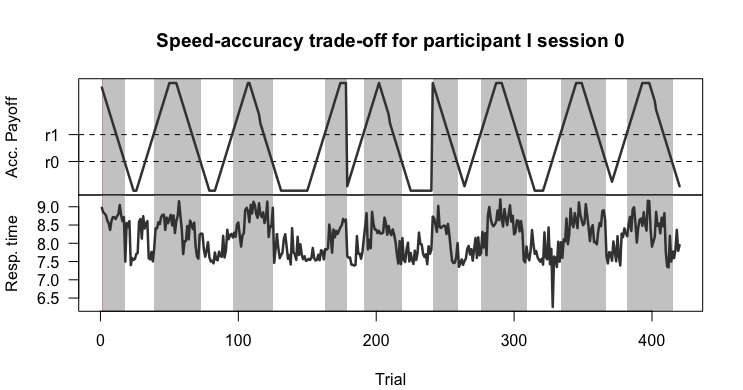
\includegraphics[scale=.5]{ts_plot_SAT}
\caption{\textit{Time series plot of response time as the outcome variable and payoff for accuracy as the control variable in a speed-accuracy trade-off experiment. The guess regime is in white and the stimulus-controlled regime is in grey.}}
\label{fig:ts_plot_SAT}
\end{center}
\end{figure}

For all $\phi$-estimates, $p < .05$. 
The mean log response time is $5.98/(1 - 0.23) = 7.77$ in the guessing regime ($R_t = \mathrm{G}$) and $3.54/(1 - 0.58) = 8.51$ in the stimulus-controlled regime ($R_t = \mathrm{SC}$). 
Note that the autoregressive effect of response times from one moment to the next is larger in the stimulus-controlled regime, indicating that the regimes are qualitatively different in their dynamics, additional to the difference in their means. This could be the case because guessing behavior is more basic and reflexive, so its variability may be less systematic. In contrast, stimulus controlled behavior is characterized by cognitive processes that could be influenced more by past trials.

\section{Discussion} \label{sec:discussion}
We presented the hysteretic threshold autoregressive (HysTAR) model \citep{bar1, bar2} to study hysteresis in univariate psychological processes characterized by two regimes.
This model can be estimated with the accompanying \textsf{R}-package \texttt{hystar} \citep{R, R_hystar}.
To the authors' knowledge, this is the first study to apply the HysTAR model to psychological time series.
With simulations, it is demonstrated that information criteria can distinguish the HysTAR model from a TAR model when the regimes differ in their means. Additionally, the Ljung-Box test can be conducted on the residuals of both models, and show a great positive predictive value when the regimes differ in their means.
Dynamic differences were found between depression network regimes and between guessing and stimulus-controlled regimes of response times, captured by the autoregressive parameters of the HysTAR model. These differences are not modeled in existing methods to study hysteresis, like the cusp catastrophe model and the hidden Markov model (HMM).
Additionally, the HysTAR model is well suited for time series data, whereas the cusp model is not applicable to time series data in its current implementations.

The HysTAR model has also limitations. 
First, it does not distinguish measurement noise from process noise, in contrast to the MSEM-RS approximation to the cusp catastrophe model \citep{chow2014regime}.
Second, the regimes only define the process of one outcome variable, whereas multiple outcomes are easily incorporated in the MSEM-RS, cusp model and HMM.

Therefore, it should be noted that various extensions of this model exist. 
For example, the Hysteretic VAR model proposed by \citet{chen} allows for multiple outcome variables. 
When there are multiple control variables, an alternative to the HysTAR model is the multivariate Hysteretic AR (MHAR) model proposed by \citet{tsay}. 
In the MHAR model, multiple control variables all have their own threshold and the regime of $y_t$ only switches when all control variables have crossed their threshold. 

Other extensions to the HysTAR model could be developed in the future.
First, it would be interesting to incorporate a second control variable in the HysTAR model, analogous to the splitting variable of the cusp catastrophe model that controls whether hysteresis present.
Such a variable could be straightforwardly implemented by adding an additional ``layer'' to the regime switching rule.
Second, a multilevel extension can be developed to investigate individual differences, which does exist for the TAR model \citep{tar_affect_dyadic1}.
Third, furture research could explore the use of an Markov switching AR (MSAR) model in the study of hysteresis, which is similar to the hidden Markov model proposed by \citet{speedaccuracy}, but also specifies and AR process for the outcome variable.

Finally, we like to stress that we think the HysTAR model should be primarily used to detect hysteresis.
The HysTAR model does not really explain anything about the mechanics underlying the hysteresis effect.
For this purpose, we need to formulate and test formal models that represent the systems underlying the hysteretic process. Then, the HysTAR model can be useful to confirm that a formal model can produce the hysteresis effect.

\paragraph{Acknowledgements}
This study is part of a project that has received funding from the European Research Council (ERC) under the European Union's Horizon 2020 research and innovation programme (grant agreement No xxxx).
\paragraph{Materials} All code to reproduce the simulation studies, empirical analyses, and figures presented in the main text are available from \url{https://github.com/daandejongen/hysteresis_paper}.

\bibliographystyle{apacite}
\bibliography{references.bib}

\appendix
 
\section{Least squares estimation of $\phi$ given $r$ and $d$}

\subsection{Estimation} \label{app:estimation}
Let $y = (y_k, \dots, y_T)$.
Let
$$X := \begin{pmatrix}
1 - R_k & (1 - R_k) y_{p_0} &  \dots & (1 - R_k) y_1 &
R_k & R_k y_{p_1} & \dots & R_k y_1 \\
1 - R_{k+1} & (1 - R_{k+1}) y_{p_0+1} & \dots & (1 - R_{k+1}) y_2 &
R_{k+1} & R_{k+1} y_{p_1+1} & \dots & R_{k+1} y_2 \\
\vdots & \vdots & \ddots & \vdots & 
\vdots & \vdots & \ddots & \vdots \\
1 - R_T & (1 - R_T) y_T & \dots & (1 - R_T) y_{T-p_0} &
R_T & R_T y_T & \dots & R_T y_{T-p_1} \\
\end{pmatrix}$$

denote the design matrix and let
$\hat{\phi} = (\hat{\phi}_{00}, \dots, \hat{\phi}_{0 p_0}, \hat{\phi}_{10}, \dots, \hat{\phi}_{1 p_1})^\prime$
denote the intercepts and AR coefficients, where $\prime$ denotes the transpose.

Then, the sum of squared errors 
$$L(\hat{\phi}, r, d) = (y - X \hat{\phi})^\prime (y - X \hat{\phi})$$
is minimized by

$$\hat{\phi} = \argmin\limits_{\phi} L(\phi, r, d) = 
(X^\prime X)^{-1} X^\prime y.$$

\subsection{Inference} \label{app:inference}
\textcolor{red}{Ik moet dit nog even beter opschrijven. Het is te doen, maar ik heb er iets meer tijd voor nodig, want het zit blijkbaar toch iets ingewikkelder dan hieronder staat.}

Let $\phi$ denote the true parameter of coefficients. Let $x_t = (1, y_{t-1}, \dots, y_{t-p})$.
Then, under Assumptions 1-4 mentioned in \textit{Section 3.2} in \citet{bar2}, 
$$T^{-\frac{1}{2}} (\hat{\phi} - \phi) \rightarrow \mathcal{N} \left( 0, \mathrm{diag}(\sigma_0^2 \Sigma_0^{-1}, \sigma_1^2 \Sigma_1^{-1}) \right)$$
in distribution as $T \rightarrow \infty$, where
$\Sigma_0^{-1} = \E[x_t x_t^\prime (1-R_t)]$ and 
$\Sigma_1^{-1} = \E[x_t x_t^\prime R_t].$

The 95\% confidence intervals of are obtained by
$\hat{\phi} - 1.96 \sqrt{\mathrm{diag}(\sigma_0^2 \Sigma_0^{-1}, \sigma_1^2 \Sigma_1^{-1})}$ as the lower bound and 
$\hat{\phi} + 1.96 \sqrt{\mathrm{diag}(\sigma_0^2 \Sigma_0^{-1}, \sigma_1^2 \Sigma_1^{-1})}$ as the upper bound.

\section{Results from SAT experiment}
\label{app:results_SAT}

\begin{table}[h!]
\begin{center}
\begin{tabular}{ l  c c  c c c c c c }
\hline
 & 
 \multicolumn{2}{c}{Part. 1, Session 1} 
 & \multicolumn{2}{c}{Part. 1, Session 2} 
 & \multicolumn{2}{c}{Part. 2, Session 1} 
 & \multicolumn{2}{c}{Part. 2, Session 2} \\
 \cline{2-9}
Parameter 
& Est. & 95\% CI 
& Est. & 95\% CI 
& Est. & 95\% CI 
& Est. & 95\% CI \\ 
\hline
$\phi_{00}$ 
& 7.28 & $[6.46, 8.11]$ 
& 4.82 & $[4.05, 5.59]$ 
& 5.98 & $[4.93, 7.03]$
& 6.26 & $[5.27, 7.26]$ \\
$\phi_{01}$ 
& 0.08 & $[-0.03, 0.18]$ 
& 0.38 & $[0.28, 0.48]$
& 0.23 & $[0.10, 0.37]$
& 0.20 & $[0.07, 0.32]$ \\
$\phi_{10}$ 
& 5.21 & $[4.44, 5.97]$ 
& 5.51 & $[4.73, 6.29]$
& 3.54 & $[2.68, 4.40]$
& 4.72 & $[3.96, 5.48]$ \\
$\phi_{11}$ 
& 0.39 & $[0.30, 0.48]$ 
& 0.35 & $[0.26, 0.44]$
& 0.58 & $[0.48, 0.68]$
& 0.44 & $[0.35, 0.53]$ \\
$r_0$ 
& 8.5 & - 
& 10.5 & -  
& 6.5 & -  
& 9.5 & - \\
$r_1$ 
& 10.5 & - 
& 11.5 & -
& 12.5 & -
& 11.5 & - \\
$d$ 
& 0 & - 
& 0 & -
& 0 & -
& 0 & -\\
$\sigma_0$ 
& 0.06 & - 
& 0.05 & -
& 0.11 & -
& 0.13 & - \\
$\sigma_1$ 
& 0.07 & - 
& 0.04 & - 
& 0.10 & - 
& 0.10 & - \\
\multicolumn{9}{c}{Information criteria} \\
\hline
Criterium 	& TAR 	& HysTAR 	& TAR 	& HysTAR 	& TAR 	& HysTAR 	& TAR 	& HysTAR \\
\hline
AIC 			& -1845 	& -1853 		& -1532 	& -1562 	 	& -919	& -921		& -1185	& -1194  \\
AICc 		& -1845 	& -1853 		& -1531 	& -1562 		& -919	& -921		& -1185	& -1194  \\
BIC 			& -1822 	& -1830 		& -1511	& -1541		& -899	& -901		& -1163 & -1173  \\
AICcp 		& -1839 	& -1841 		& -1526 	& -1540 	 	& -913	& -909		& -1179	& -1182  \\
\hline
\end{tabular}
\caption{Point estimates and confidence intervals of the parameters of the HysTAR model for participants and sessions. Additionally, the table presents estimates of information criteria for the TAR and HysTAR model, where a lower value indicates preference of one model over the other.}
\end{center}
\end{table}

\begin{figure}
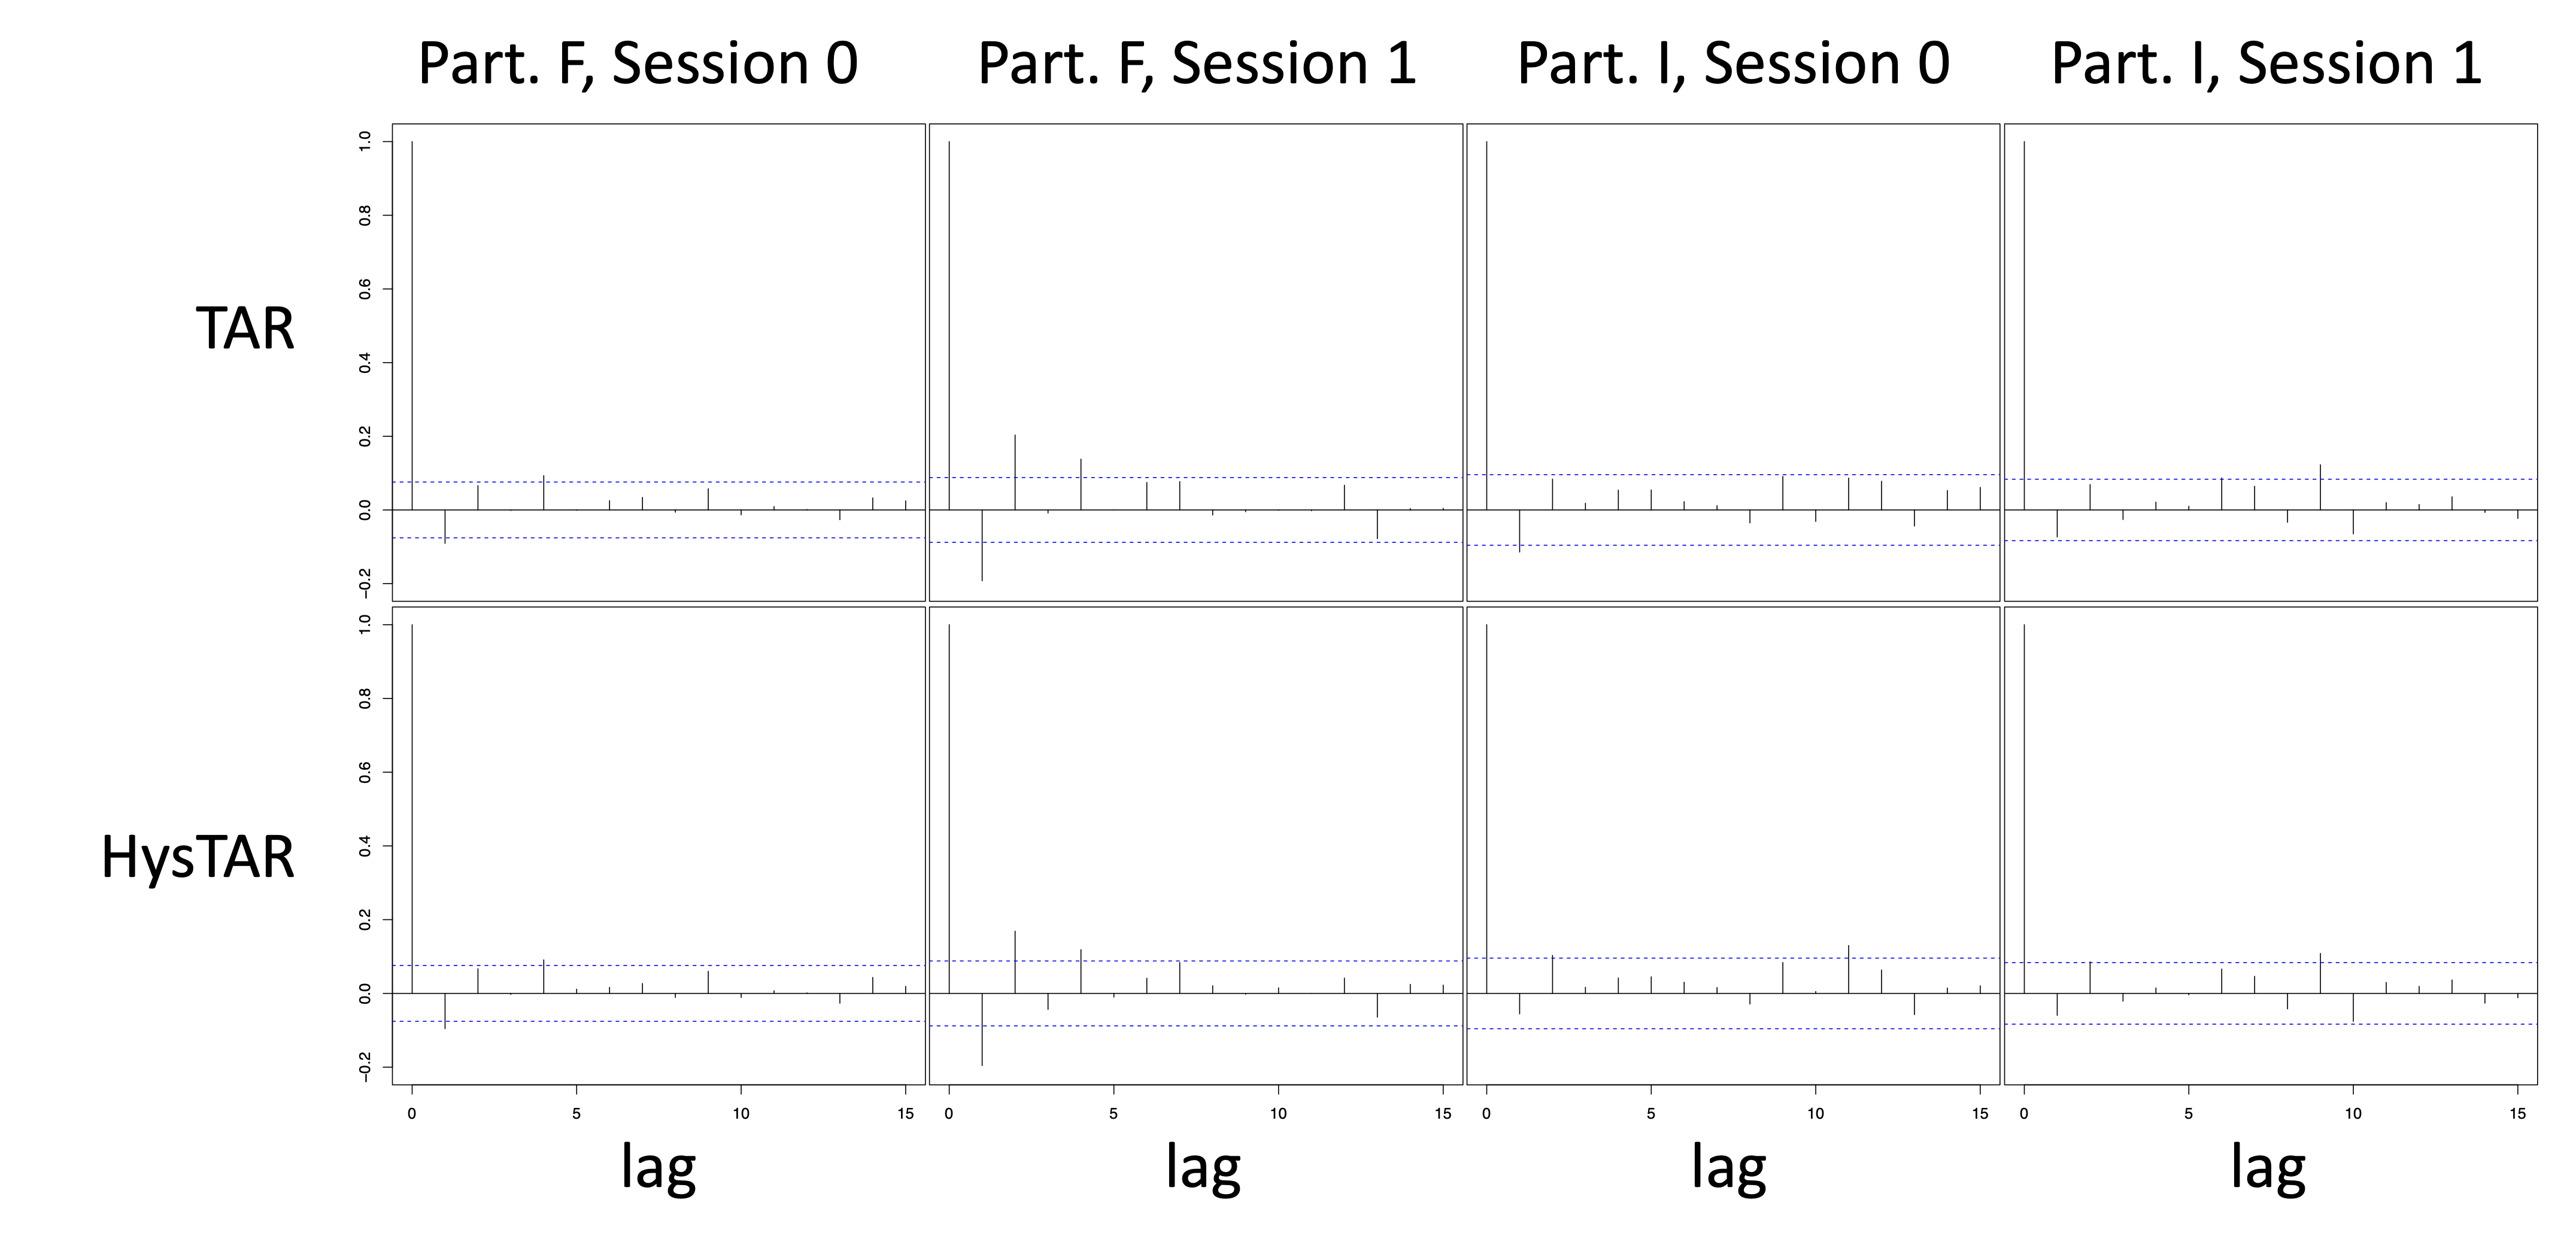
\includegraphics[scale=.5]{resplots_SAT}
\caption{Estimated ACFs of the residuals from the TAR and HysTAR model, for all sessions. The dashed lines represent the 95\% confidence interval around 0.}
\end{figure}

%\end{multicols}

\end{document}
